% SPDX-License-Identifier: MPL-2.0
%
% Binary Star: A Neurosymbolic IDE Architecture with Cognitive Governance
% and Constraint-Validated Human-AI Co-Orbit
%
% Jonathan D.A. Jewell, 2026

\documentclass[11pt,a4paper]{article}

% ---------- packages ----------
\usepackage[utf8]{inputenc}
\usepackage[T1]{fontenc}
\usepackage{lmodern}
\usepackage{amsmath,amssymb,amsthm}
\usepackage{mathtools}
\usepackage{stmaryrd}
\usepackage{graphicx}
\usepackage{booktabs}
\usepackage{enumitem}
\usepackage{hyperref}
\usepackage{cleveref}
\usepackage{xcolor}
\usepackage{tikz}
\usetikzlibrary{arrows.meta,positioning,calc,decorations.pathmorphing,shapes.geometric}
\usepackage{algorithm}
\usepackage{algpseudocode}
\usepackage[margin=1in]{geometry}
\usepackage{microtype}
\usepackage{natbib}
\bibliographystyle{plainnat}

% ---------- theorem environments ----------
\newtheorem{definition}{Definition}[section]
\newtheorem{proposition}{Proposition}[section]
\newtheorem{invariant}{Invariant}[section]
\newtheorem{property}{Property}[section]
\newtheorem{theorem}{Theorem}[section]

% ---------- custom commands ----------
\newcommand{\paneL}{\textsc{Pane-L}}
\newcommand{\paneN}{\textsc{Pane-N}}
\newcommand{\paneW}{\textsc{Pane-W}}
\newcommand{\panll}{\textsc{PanLL}}
\newcommand{\typell}{\textsc{TypeLL}}
\newcommand{\ensaid}{\textsc{eNSAID}}
\newcommand{\tea}{\textsc{TEA}}
\newcommand{\ooda}{\textsc{OODA}}

\title{Binary Star: A Neurosymbolic IDE Architecture\\with Cognitive Governance and\\Constraint-Validated Human-AI Co-Orbit}

\author{Jonathan D.A. Jewell\\
\textit{Independent Researcher}\\
\texttt{j.d.a.jewell@open.ac.uk}}

\date{March 2026}

\begin{document}

\maketitle

% ============================================================
%  ABSTRACT
% ============================================================
\begin{abstract}
Contemporary AI-assisted development environments operate under an
implicit master--servant topology: the human commands, the machine
obeys. This asymmetry produces characteristic failure modes---unchecked
neural hallucination, opaque reasoning, cognitive overload from
undifferentiated suggestion streams, and an absence of formal
guarantees on the boundary between human intent and machine output.
We present \panll{} (\textit{Parallel}), an \ensaid{} (Environment
for NeSy-Agentic Integrated Development) that replaces the
master--servant model with a \textit{Binary Star} architecture in
which the human operator and the neurosymbolic machine co-orbit a
shared task barycentre. The architecture is realised through three
principal contributions: (1)~a three-pane layout (\paneL{}/\paneN{}/\paneW{})
in which symbolic constraints, neural reasoning, and validated results
occupy distinct but gravitationally coupled regions; (2)~six cognitive
governance subsystems that maintain orbital stability through
frustration tracking, information density adaptation, constraint
validation gates, drift detection, elastic state contracts, and
cross-pane synchronisation monitoring; and (3)~\typell{}, an invisible
dependent-type verification backbone that type-checks neural and
symbolic outputs against each other before results enter the shared
workspace. The system is implemented in ReScript with The Elm
Architecture for state management, a Rust/Gossamer backend (Zig + WebKitGTK for a lightweight,
container-friendly webview shell), and an
Elixir/BEAM middleware layer, comprising over 500 source files across
79 panel modules. We describe the formal properties of the Binary Star
model, detail each governance subsystem with its invariants, and
discuss the architectural implications for human-AI co-creation
environments.
\end{abstract}

\vspace{0.5em}
\noindent\textbf{Keywords:} neurosymbolic computing, human-AI interaction,
cognitive governance, constraint satisfaction, IDE architecture,
binary star model, dependent types, The Elm Architecture

% ============================================================
%  1. INTRODUCTION
% ============================================================
\section{Introduction}\label{sec:intro}

The last four years have seen AI-assisted programming move from
research curiosity to daily practice. Tools such as GitHub
Copilot~\citep{chen2021evaluating}, Cursor, and Cody provide
inline code completions, chat-based code generation, and
increasingly agentic multi-file editing capabilities. These systems
share an implicit architectural assumption: the human is the
principal, the AI is the agent. The human describes intent; the
machine produces artefacts; the human accepts or rejects.

This principal--agent framing, which we term the \textit{master--servant
topology}, has been productive but carries structural limitations
that become pronounced as AI capabilities increase:

\begin{enumerate}[label=(\roman*)]
  \item \textbf{Unchecked neural output.} Suggestions arrive in the
    workspace without passing through any formal validation gate. The
    human must serve as the sole verification layer.
  \item \textbf{Opaque reasoning.} The machine's internal deliberation
    ---its confidence levels, alternative paths considered, causal
    chains---is invisible. The human cannot inspect \textit{why} a
    suggestion was produced, only \textit{what} was produced.
  \item \textbf{Cognitive overload.} Suggestion streams arrive at
    uniform density regardless of the operator's current cognitive
    state, task complexity, or frustration level.
  \item \textbf{No symmetry of constraint.} The human's formal
    requirements (type signatures, invariants, proof obligations) and
    the machine's reasoning are not subject to the same validation
    regime. They exist in separate, unconnected spaces.
\end{enumerate}

We argue that these are not incidental deficiencies but structural
consequences of the master--servant topology itself. An alternative
is needed---not one that inverts the hierarchy (machine commands,
human obeys) but one that dissolves it.

\subsection{The Binary Star Hypothesis}

In astrophysics, a binary star system consists of two stellar bodies
orbiting a shared centre of mass (barycentre). Neither body dominates;
both are constrained by the gravitational field they jointly produce.
The system's stability depends on each body maintaining its orbital
parameters relative to the barycentre, not relative to each other.

We propose that productive human-AI co-creation exhibits analogous
dynamics. The shared \textit{task}---with its constraints, requirements,
and validation criteria---functions as the gravitational centre. Both
the human operator and the machine are constrained by the task's
``gravity.'' Neither dictates to the other; both contribute mass
(constraints and inferences, respectively) that shapes the shared
field.

\panll{} is an implementation of this hypothesis. It is an \ensaid{}---an
Environment for NeSy-Agentic Integrated Development---designed to
make the co-orbit visible, governable, and formally constrained.

\subsection{Contributions}

This paper makes the following contributions:

\begin{enumerate}
  \item A formal model of the Binary Star architecture, including its
    symmetry properties, stability conditions, and relationship to
    constraint satisfaction (\Cref{sec:binary-star}).
  \item The three-pane (L/N/W) layout that spatially separates symbolic
    mass, neural stream, and world state while maintaining
    gravitational coupling through typed message passing
    (\Cref{sec:three-pane}).
  \item Six cognitive governance subsystems with formal definitions and
    invariants (\Cref{sec:governance}).
  \item \typell{}, a cross-panel dependent type verification kernel
    (\Cref{sec:typell}).
  \item A constraint-driven five-phase architecture from substrate
    through observability (\Cref{sec:constraint-propagation}).
  \item An implementation report covering the ReScript/Gossamer/BEAM stack
    (\Cref{sec:implementation}).
\end{enumerate}

\subsection{Scope and Limitations}

\panll{} is a personal neurosymbolic workbench, not a general-purpose
IDE framework. The evaluation is qualitative and architectural rather
than based on controlled user studies. We make no claims of
superiority over existing tools for conventional programming tasks;
our interest is in the structural properties of the human-AI
interaction topology and their consequences for cognitive ergonomics
and formal assurance.

% ============================================================
%  2. BACKGROUND
% ============================================================
\section{Background and Related Work}\label{sec:background}

\subsection{AI Pair Programming}

The dominant paradigm for AI-assisted development descends from
language model code completion. \citet{chen2021evaluating} introduced
Codex and its productisation as GitHub Copilot, establishing the
inline-suggestion model that subsequent tools have refined. Cursor
extends this with multi-file awareness and agentic editing.
Amazon CodeWhisperer, Cody (Sourcegraph), and Tabnine offer
variations on the theme. All share the master--servant topology:
the human drives, the AI suggests.

Recent work on AI agents (SWE-Agent~\citep{yang2024sweagent},
Devin, Claude Code) pushes toward greater machine autonomy, but
the underlying topology remains asymmetric. The agent proposes
changes; the human approves or rejects. There is no shared
constraint space, no visibility into reasoning, and no formal
governance of the interaction.

\subsection{Neurosymbolic Computing}

Neurosymbolic AI combines neural learning with symbolic
reasoning~\citep{garcez2023neurosymbolic}. In the programming
domain, this manifests as systems that combine neural code
generation with type checking, formal verification, or constraint
satisfaction. \citet{jha2010oracle} introduced oracle-guided
inductive synthesis, where a formal specification constrains the
space of acceptable programs. More recently, LLM-guided proof
search~\citep{first2023baldur} demonstrates tight coupling between
neural generation and symbolic verification.

\panll{} differs from these approaches in that it does not combine
neural and symbolic reasoning within a single inference pipeline.
Instead, it \textit{spatially separates} them into distinct panes
and imposes a validation gate between the neural stream and the
shared workspace. The neurosymbolic property emerges from the
architecture's topology, not from a hybrid model.

\subsection{Cognitive Load Theory}

\citet{sweller1988cognitive} established that learning and
performance degrade when cognitive load exceeds working memory
capacity. In software development, \citet{fritz2014using}
demonstrated correlations between biometric signals and
perceived task difficulty. The concept of ``flow''
\citep{csikszentmihalyi1990flow} describes optimal engagement
states characterised by balanced challenge and skill.

AI-assisted development tools have largely ignored cognitive load
as a design variable. Suggestion streams arrive at constant density
regardless of operator state. \panll{}'s cognitive governance
subsystems---particularly the Vexometer and Information Humidity
systems---treat cognitive load as a first-class architectural concern.

\subsection{Constraint Satisfaction in IDEs}

Type systems, linters, and static analysers implement constraint
checking within development environments, but typically operate
post-hoc: the developer writes code, the tool reports violations.
Constraint propagation~\citep{mackworth1977consistency} from the
constraint satisfaction literature offers a more active model in
which constraints propagate through a network, pruning the space
of acceptable states before violations occur.

The Binary Star model incorporates constraint propagation as its
fundamental interaction mechanism. Symbolic constraints in \paneL{}
propagate through the validation gate to constrain what neural output
can reach \paneW{}, rather than flagging violations after the fact.

\subsection{The Elm Architecture}

The Elm Architecture (\tea{})~\citep{czaplicki2012elm} provides a
purely functional state management pattern: a single immutable
\texttt{Model}, typed \texttt{Msg} values representing all possible
state transitions, and a pure \texttt{update} function. Originally
developed for the Elm programming language, \tea{} has influenced
React/Redux and similar frameworks but is rarely adopted in its
pure form outside Elm itself.

\panll{} implements \tea{} in ReScript, exploiting ReScript's sound
type system to enforce exhaustive pattern matching on all message
variants. With over 50 model slices and hundreds of message types,
adding a new variant to any model triggers compiler errors at every
unhandled case---a property that TypeScript's structural type system
cannot provide with the same rigour.

% ============================================================
%  3. THE BINARY STAR MODEL
% ============================================================
\section{The Binary Star Model}\label{sec:binary-star}

\subsection{Informal Description}

In the Binary Star model, the human operator ($H$) and the
neurosymbolic machine ($M$) co-orbit a shared task barycentre ($B$).
The barycentre is not controlled by either party; it is the
weighted centre of their combined contributions. $H$ contributes
\textit{symbolic mass}---formal constraints, type signatures, proof
obligations, acceptance criteria. $M$ contributes \textit{neural
mass}---generated code, inferred types, suggested refactorings,
reasoning traces. The barycentre $B$ contains only \textit{validated
results}---outputs that have passed through both symbolic and neural
validation.

\begin{figure}[t]
\centering
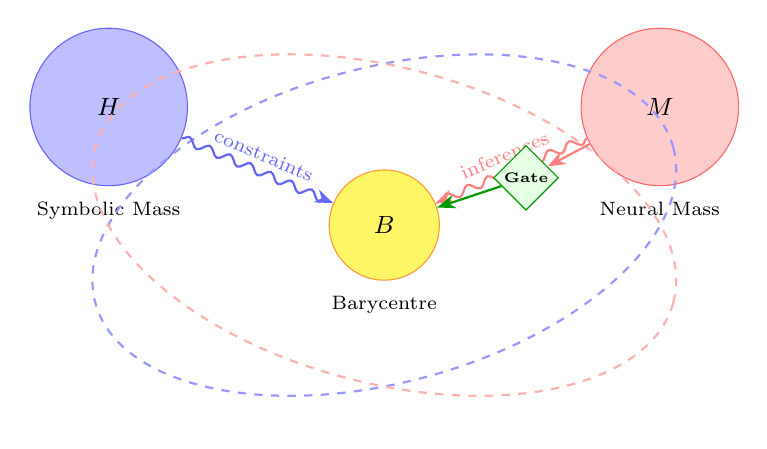
\begin{tikzpicture}[>=Stealth, scale=1.0]
  % Barycentre
  \node[circle, fill=yellow!60, draw=orange!80, minimum size=1.4cm,
        font=\small\bfseries] (B) at (0,0) {$B$};
  \node[below=2pt of B, font=\scriptsize] {Barycentre};

  % Human
  \node[circle, fill=blue!25, draw=blue!60, minimum size=2.0cm,
        font=\small\bfseries] (H) at (-3.5,1.5) {$H$};
  \node[below=2pt of H, font=\scriptsize] {Symbolic Mass};

  % Machine
  \node[circle, fill=red!20, draw=red!60, minimum size=2.0cm,
        font=\small\bfseries] (M) at (3.5,1.5) {$M$};
  \node[below=2pt of M, font=\scriptsize] {Neural Mass};

  % Orbital paths (dashed ellipses)
  \draw[blue!40, dashed, thick, rotate around={15:(0,0)}]
    (0,0) ellipse (3.8cm and 2.0cm);
  \draw[red!30, dashed, thick, rotate around={-15:(0,0)}]
    (0,0) ellipse (3.8cm and 2.0cm);

  % Gravitational arrows
  \draw[->, thick, blue!60, decorate,
        decoration={snake, amplitude=1.5pt, segment length=8pt}]
    (H) -- (B) node[midway, above, font=\scriptsize, sloped] {constraints};
  \draw[->, thick, red!50, decorate,
        decoration={snake, amplitude=1.5pt, segment length=8pt}]
    (M) -- (B) node[midway, above, font=\scriptsize, sloped] {inferences};

  % Validation gate
  \node[diamond, draw=green!60!black, fill=green!10, minimum size=0.8cm,
        font=\tiny\bfseries, inner sep=1pt] (G) at (1.8, 0.6) {Gate};
  \draw[->, thick, red!50] (M) -- (G);
  \draw[->, thick, green!60!black] (G) -- (B);
\end{tikzpicture}
\caption{The Binary Star model. Human ($H$) and Machine ($M$) co-orbit
the task barycentre ($B$). Neural inferences must pass through the
validation gate before reaching $B$.}
\label{fig:binary-star}
\end{figure}

\subsection{Formal Definition}

\begin{definition}[Binary Star System]\label{def:binary-star}
A \textit{Binary Star System} is a tuple
$\mathcal{S} = (H, M, B, \Gamma, \Delta, \phi)$ where:
\begin{itemize}
  \item $H = (\Sigma, \mathcal{C})$ is the human component,
    with symbolic state $\Sigma$ and constraint set
    $\mathcal{C} \subseteq \mathcal{P}(\text{Prop})$.
  \item $M = (\mathcal{N}, \Theta)$ is the machine component,
    with neural state $\mathcal{N}$ and confidence distribution
    $\Theta : \mathcal{N} \to [0,1]$.
  \item $B \subseteq \mathcal{V}$ is the barycentre (validated
    result set), where $\mathcal{V}$ is the space of valid artefacts.
  \item $\Gamma : \mathcal{N} \times \mathcal{C} \to
    \{\texttt{Valid}, \texttt{Invalid}, \texttt{Review}\}$ is the
    \textit{Anti-Crash gate} function.
  \item $\Delta : H \times M \to [0,1]$ is the \textit{divergence
    metric} measuring orbital drift.
  \item $\phi : B \times H \times M \to B$ is the barycentre
    update function, satisfying $\phi(B, H, M) \supseteq B$ (monotonic
    growth of validated results under stable orbits).
\end{itemize}
\end{definition}

\begin{invariant}[Gate Exclusion]\label{inv:gate}
No neural output $n \in \mathcal{N}$ enters the barycentre $B$ without
satisfying $\Gamma(n, \mathcal{C}) = \texttt{Valid}$:
\[
  \forall n \in \mathcal{N}.\; n \in B \implies
    \Gamma(n, \mathcal{C}) = \texttt{Valid}
\]
\end{invariant}

\begin{property}[Orbital Symmetry]\label{prop:symmetry}
Both $H$ and $M$ are subject to the task's constraints. The operator's
symbolic contributions are type-checked by \typell{}; the machine's
neural contributions are validated by the Anti-Crash gate.
Neither component has unvalidated write access to $B$.
\end{property}

\begin{property}[Divergence Boundedness]\label{prop:divergence}
The system maintains a divergence bound $\delta_{\max}$ such that if
$\Delta(H, M) > \delta_{\max}$, governance interventions are triggered
(see \Cref{sec:governance}). This prevents unbounded orbital drift
where the human and machine work on increasingly unrelated tasks.
\end{property}

\subsection{Comparison with the Master--Servant Topology}

In the master--servant topology, the interaction reduces to a
function $f: \text{Intent} \to \text{Artefact}$ where the human
provides intent and the machine returns artefacts. This model
lacks:

\begin{itemize}
  \item A shared validated space ($B$ does not exist; outputs go
    directly to the workspace).
  \item A gate function ($\Gamma$ is absent; the human is the sole
    validator).
  \item A divergence metric ($\Delta$ is undefined; there is no
    concept of drift between human and machine state).
  \item Bidirectional constraint ($H$ constrains $M$ but $M$ does
    not constrain $H$).
\end{itemize}

The Binary Star model addresses all four gaps. The cost is
architectural complexity: maintaining three panes, six governance
subsystems, and a type-checking kernel is more involved than a
single-pane editor with an inline suggestion stream.

% ============================================================
%  4. THREE-PANE ARCHITECTURE
% ============================================================
\section{Three-Pane Architecture}\label{sec:three-pane}

The Binary Star model is spatially realised through three panes,
each corresponding to a component of the system.

\subsection{Pane-L: Symbolic Mass}

\paneL{} houses the human operator's formal contributions:
type constraints, property specifications, proof obligations, and
acceptance criteria. It is the \textit{law} that governs neural
inference---no output reaches the workspace unless it satisfies
the constraints expressed here.

\begin{definition}[Symbolic Constraint]\label{def:constraint}
A symbolic constraint $c \in \mathcal{C}$ is a triple
$(e, a, d)$ where $e$ is a constraint expression (a predicate
over artefacts), $a \in \{\texttt{true}, \texttt{false}\}$ is
the activation flag, and $d$ is an optional human-readable
description.
\end{definition}

In the implementation, constraints include type declarations,
forbidden-pattern exclusions (e.g., $\lnot\texttt{contains}(\text{``eval''})$),
and structural requirements. The constraint set $\mathcal{C}$ is
persisted and restored across sessions.

\subsection{Pane-N: Neural Stream}

\paneN{} makes the machine's reasoning visible. Rather than
presenting only final outputs (as in the master--servant model),
\paneN{} exposes:

\begin{itemize}
  \item \textbf{Token stream:} The raw sequence of neural outputs,
    before validation.
  \item \textbf{OODA phases:} The machine's position in the
    Observe--Orient--Decide--Act
    loop~\citep{boyd1996essence}, making its deliberation
    cycle legible.
  \item \textbf{Internal monologue:} A natural-language trace of
    the machine's reasoning process.
  \item \textbf{Confidence distribution:} Per-token confidence
    scores $\Theta(n)$ for each neural output $n$.
  \item \textbf{Causal chains:} The dependency structure connecting
    observations to decisions.
\end{itemize}

Crucially, \paneN{} also hosts the ECHIDNA theorem prover
dispatch panel, which provides access to 30 solver backends
(including Z3, CVC5, E, and Lean) for interactive proof
construction. Proofs in \paneN{} generate trust certificates
that propagate to \paneW{}.

\begin{definition}[Trust Level Hierarchy]\label{def:trust}
ECHIDNA assigns a 5-tier trust level to each verified result:
\begin{enumerate}
  \item[\textbf{L1}] Single unverified solver, high axiom risk.
  \item[\textbf{L2}] Single solver, no dangerous axioms.
  \item[\textbf{L3}] Multiple solvers agree.
  \item[\textbf{L4}] Cross-checked, no axiom issues.
  \item[\textbf{L5}] Full formal proof, cross-checked, certificate issued.
\end{enumerate}
Dangerous axioms---\texttt{believe\_me}, \texttt{Admitted},
\texttt{sorry}, \texttt{unsafeCoerce}, \texttt{Obj.magic}---are
classified at three danger levels: \texttt{Noted} (standard
library, informational), \texttt{Warning} (potentially unsound),
and \texttt{Reject} (proof-breaking).
\end{definition}

\subsection{Pane-W: The Barycentre}

\paneW{} is the shared validated result space---the world that both
$H$ and $M$ can see and modify, but only through their respective
validation gates. It corresponds to $B$ in \Cref{def:binary-star}.

Content enters \paneW{} through two paths:
\begin{enumerate}
  \item \textbf{Neural path:} $M \xrightarrow{\text{token}} \Gamma
    \xrightarrow{\texttt{Valid}} B$. Neural tokens pass through the
    Anti-Crash gate, which validates them against \paneL{} constraints.
  \item \textbf{Symbolic path:} $H \xrightarrow{\text{constraint}}
    \typell{} \xrightarrow{\text{checked}} B$. Human contributions
    are type-checked by the \typell{} kernel before entering the
    workspace.
\end{enumerate}

Both paths enforce \Cref{inv:gate}: nothing enters $B$ unvalidated.

\subsection{Data Flow}

\begin{figure}[t]
\centering
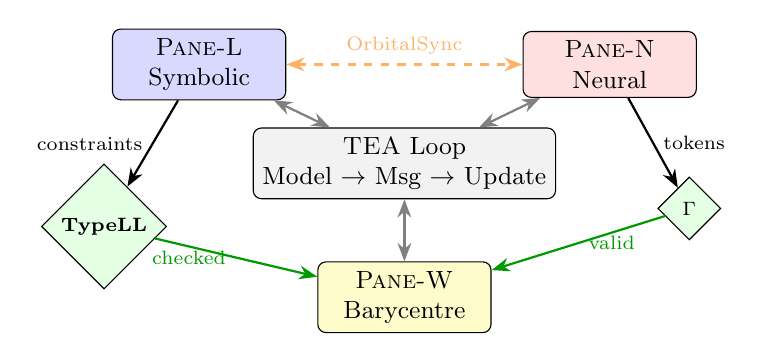
\begin{tikzpicture}[>=Stealth, node distance=1.5cm and 2.5cm,
  box/.style={rectangle, draw, rounded corners=3pt, minimum width=2.2cm,
              minimum height=0.8cm, font=\small, align=center},
  gate/.style={diamond, draw, fill=green!10, minimum size=0.8cm,
               font=\scriptsize\bfseries, inner sep=2pt}]

  % Panes
  \node[box, fill=blue!15] (L) {\paneL{}\\Symbolic};
  \node[box, fill=red!12, right=3cm of L] (N) {\paneN{}\\Neural};
  \node[box, fill=yellow!20, below=2.5cm of $(L)!0.5!(N)$] (W)
    {\paneW{}\\Barycentre};

  % Gates
  \node[gate, below right=1.2cm and -0.3cm of N] (G1) {$\Gamma$};
  \node[gate, below left=1.2cm and -0.3cm of L] (G2) {\typell{}};

  % TEA loop
  \node[box, fill=gray!10, below=0.8cm of $(L)!0.5!(N)$] (TEA)
    {\tea{} Loop\\Model $\to$ Msg $\to$ Update};

  % Arrows
  \draw[->, thick] (N) -- (G1) node[midway, right, font=\scriptsize] {tokens};
  \draw[->, thick, green!60!black] (G1) -- (W) node[midway, right, font=\scriptsize] {valid};
  \draw[->, thick] (L) -- (G2) node[midway, left, font=\scriptsize] {constraints};
  \draw[->, thick, green!60!black] (G2) -- (W) node[midway, left, font=\scriptsize] {checked};
  \draw[<->, thick, gray] (L) -- (TEA);
  \draw[<->, thick, gray] (N) -- (TEA);
  \draw[<->, thick, gray] (TEA) -- (W);

  % Cross-pane sync
  \draw[<->, dashed, orange!60, thick] (L) -- (N)
    node[midway, above, font=\scriptsize] {OrbitalSync};
\end{tikzpicture}
\caption{Three-pane data flow. All state changes pass through the
\tea{} loop. Neural tokens are gated by $\Gamma$; symbolic contributions
are checked by \typell{}. OrbitalSync monitors cross-pane divergence.}
\label{fig:three-pane}
\end{figure}

All state transitions in the system pass through the \tea{} update
loop (\Cref{fig:three-pane}). Each pane dispatches typed messages;
the pure \texttt{update} function routes them, applies validation,
and produces the next immutable model state. There is no mutable
global state, no event emitters with implicit coupling, and no
callback-based side effects. Commands (Gossamer IPC calls, HTTP
requests, filesystem operations) are described as data and executed
by the runtime, following the command pattern from the original
Elm Architecture~\citep{czaplicki2012elm}.

% ============================================================
%  5. COGNITIVE GOVERNANCE
% ============================================================
\section{Cognitive Governance}\label{sec:governance}

The six cognitive governance subsystems maintain orbital stability
by monitoring and adjusting the interaction between $H$, $M$, and
$B$. Each subsystem operates as a pure function over the \tea{}
model, producing messages that trigger governance interventions.

\subsection{Anti-Crash Gate}

The Anti-Crash gate implements the function $\Gamma$ from
\Cref{def:binary-star}. It is a logical circuit breaker that
intercepts every neural token and validates it against the active
symbolic constraints before allowing it to reach the barycentre.

\begin{definition}[Anti-Crash Gate]\label{def:anticrash}
Let $\mathcal{C}_a = \{c \in \mathcal{C} \mid c.a = \texttt{true}\}$
be the set of active constraints. The gate function is:
\[
  \Gamma(n, \mathcal{C}_a) = \begin{cases}
    \texttt{Invalid}(c) & \text{if } \exists c \in \mathcal{C}_a.\;
      \lnot\, c.e(n) \\
    \texttt{RequiresReview}(c) & \text{if } \exists c \in \mathcal{C}_a.\;
      c.e(n) = \texttt{ambiguous} \\
    \texttt{Valid} & \text{otherwise}
  \end{cases}
\]
\end{definition}

The gate operates in two modes:
\begin{itemize}
  \item \textbf{Strict mode:} Both \texttt{Invalid} and
    \texttt{RequiresReview} results block the token. The system halts
    until the operator resolves the ambiguity.
  \item \textbf{Adaptive mode:} \texttt{RequiresReview} results are
    flagged but allowed to pass, with the operator notified
    asynchronously.
\end{itemize}

The gate maintains a violation log with timestamps, enabling
post-hoc analysis of which constraints are most frequently violated
and whether the constraint set needs refinement.

\begin{invariant}[Anti-Crash Completeness]\label{inv:anticrash}
In strict mode, the gate is a total function over the cross-product
of neural tokens and active constraints:
\[
  \forall n \in \mathcal{N},\; \forall \mathcal{C}_a.\;
    \Gamma(n, \mathcal{C}_a) \in
    \{\texttt{Valid}, \texttt{Invalid}, \texttt{RequiresReview}\}
\]
No token is silently dropped or passed without evaluation.
\end{invariant}

\subsection{Vexometer}

The Vexometer tracks operator frustration through observable proxy
signals, providing a real-time cognitive load estimate without
requiring biometric sensors.

\begin{definition}[Vexation Index]\label{def:vexometer}
The vexation index $V(t) \in [0, 1]$ at time $t$ is computed as:
\[
  V(t) = \alpha \cdot C(t) + \beta \cdot R(t) + \gamma \cdot D(t)
\]
where:
\begin{itemize}
  \item $C(t)$ is the cancellation rate (frequency of abandoned
    operations), with exponential decay $C(t) = \sum_{i} e^{-\lambda(t - t_i)}$
    over recent cancellation events $\{t_i\}$.
  \item $R(t)$ is the correction rate (frequency of undo/redo
    sequences and immediate edits to machine output).
  \item $D(t)$ is the dwell time anomaly (deviation from the
    operator's baseline interaction tempo).
  \item $\alpha + \beta + \gamma = 1$ are tunable weights.
\end{itemize}
\end{definition}

When $V(t)$ exceeds a configurable threshold $V_{\max}$, the
Vexometer triggers governance interventions: reducing suggestion
frequency, simplifying displayed information, or pausing neural
output entirely until the index subsides.

\begin{algorithm}[t]
\caption{Vexation Index Update}\label{alg:vexometer}
\begin{algorithmic}[1]
\Require Event $e$ at time $t$, current state $(V, C, R, D)$,
  decay rate $\lambda$
\Ensure Updated vexation index $V'$
\State Apply exponential decay to $C$, $R$, $D$
\If{$e$ is a cancellation}
  \State $C \gets C + 1$
\ElsIf{$e$ is a correction}
  \State $R \gets R + 1$
\ElsIf{$e$ is a dwell event}
  \State $D \gets |t - t_{\text{expected}}| / t_{\text{baseline}}$
\EndIf
\State $V' \gets \alpha \cdot C + \beta \cdot R + \gamma \cdot D$
\State Clamp $V'$ to $[0, 1]$
\If{$V' > V_{\max}$}
  \State Emit \texttt{VexationCeiling} governance message
\EndIf
\State \Return $V'$
\end{algorithmic}
\end{algorithm}

The Vexometer also computes a per-tool friction profile, measuring
how much each integrated tool contributes to overall frustration.
Tools with consistently high friction scores are flagged for UX
improvement in the Vexometer Friction panel.

\subsection{Information Humidity}

Information Humidity adapts UI density based on estimated cognitive
load, functioning as the display-layer complement to the Vexometer's
measurement layer.

\begin{definition}[Information Humidity]\label{def:humidity}
Information humidity $\mathcal{H} \in [0, 1]$ controls the density of
information displayed, where $\mathcal{H} = 0$ is minimal (``desert'')
and $\mathcal{H} = 1$ is maximal (``rainforest''). The humidity is
computed as:
\[
  \mathcal{H}(t) = \mathcal{H}_{\text{base}} \cdot (1 - V(t))
\]
where $\mathcal{H}_{\text{base}}$ is the operator's preferred baseline
density and $V(t)$ is the current vexation index.
\end{definition}

As frustration increases, humidity decreases: panels show fewer
details, confidence scores are collapsed into summary badges,
and secondary information is progressively hidden. The operator
can override humidity manually, but the automatic adjustment
provides a cognitive ``air conditioning'' effect that reduces
information overload during high-stress moments.

Humidity affects all three panes uniformly, maintaining the
principle that governance applies symmetrically to both $H$
and $M$ interfaces.

\subsection{Orbital Drift Aura}

The Orbital Drift Aura provides an ambient visual indicator of the
divergence between \paneL{} and \paneN{} content---a measure of how
far the human's constraints and the machine's reasoning have drifted
apart.

\begin{definition}[Orbital Divergence]\label{def:drift}
Let $T_L$ and $T_N$ be the token sets extracted from \paneL{} and
\paneN{} content, respectively. The orbital divergence is the
Jaccard distance:
\[
  \Delta_J(T_L, T_N) = 1 - \frac{|T_L \cap T_N|}{|T_L \cup T_N|}
\]
When both token sets are empty, divergence defaults to a
length-ratio fallback:
\[
  \Delta_{\text{len}}(\Sigma, \mathcal{N}) =
    1 - \frac{\min(|\Sigma|, |\mathcal{N}|)}{\max(|\Sigma|, |\mathcal{N}|) + 1}
\]
\end{definition}

The divergence is rendered as an ambient colour aura surrounding
the workspace:
\begin{itemize}
  \item $\Delta < 0.3$: green (tight co-orbit).
  \item $0.3 \leq \Delta < 0.6$: amber (moderate drift).
  \item $\Delta \geq 0.6$: red (significant divergence---the
    human and machine may be working on different problems).
\end{itemize}

The aura is deliberately ambient rather than intrusive. It occupies
peripheral vision, leveraging pre-attentive colour processing to
convey system state without demanding focal attention.

\begin{property}[Drift Monotonicity Warning]\label{prop:drift-mono}
If divergence increases monotonically over $k$ consecutive
measurements ($\Delta_{t+1} > \Delta_t$ for $k$ steps), the
system escalates from ambient aura to an explicit notification,
suggesting the operator review the co-orbit state.
\end{property}

\subsection{Contractiles}

Contractiles are elastic state contracts between the operator and
the machine. Unlike static contracts that are either satisfied or
violated, contractiles adapt their boundaries based on the system's
current state.

\begin{definition}[Contractile]\label{def:contractile}
A contractile is a tuple $(p, \ell, s)$ where:
\begin{itemize}
  \item $p : \text{Model} \to \texttt{Satisfied} \mid
    \texttt{Violated}(\text{reason})$ is a predicate over the
    full model state.
  \item $\ell \in \{\texttt{Strict}, \texttt{Warn},
    \texttt{Adaptive}\}$ is the enforcement level.
  \item $s$ is the current status, updated at each \tea{} cycle.
\end{itemize}
\end{definition}

The system provides four built-in contractiles:

\begin{enumerate}
  \item \textbf{Orbital Stability Bound:} Requires
    orbital stability $\geq$ a threshold. If violated, neural
    output rate is reduced.
  \item \textbf{Vexation Ceiling:} Requires vexation index
    $\leq$ a ceiling. If violated, information humidity is
    decreased.
  \item \textbf{Divergence Limit:} Requires orbital divergence
    $\leq$ a limit. If violated, cross-pane synchronisation is
    forced.
  \item \textbf{Autonomy Bound:} Requires machine autonomy level
    $\leq$ a maximum. If violated, the machine's action space is
    restricted until the operator explicitly expands it.
\end{enumerate}

Under \texttt{Adaptive} enforcement, contractile boundaries shift
based on recent history: if a bound is consistently close to
violation, it relaxes slightly; if it is consistently satisfied
with margin, it tightens. This prevents the system from oscillating
between governance interventions and quiescent states.

\subsection{Sync Health Monitor}

The Sync Health Monitor tracks cross-pane latency and data freshness,
ensuring that the three panes maintain temporal coherence.

\begin{definition}[Sync Health]\label{def:sync}
Sync health is a tuple $(h_L, h_N, h_W, \tau)$ where:
\begin{itemize}
  \item $h_L, h_N, h_W$ are content hashes for \paneL{}, \paneN{},
    \paneW{}, respectively, recomputed at each \tea{} cycle.
  \item $\tau$ is the maximum observed propagation delay between
    a state change in one pane and its reflection (if applicable)
    in another.
\end{itemize}
The monitor detects three classes of anomaly:
\begin{enumerate}
  \item \textbf{Stale pane:} A pane's hash has not changed for
    $> k$ cycles while other panes have changed.
  \item \textbf{Propagation delay:} $\tau > \tau_{\max}$,
    indicating that validated results are not reaching
    \paneW{} in a timely manner.
  \item \textbf{Phantom update:} A pane's hash changes without
    a corresponding \tea{} message, indicating a state mutation
    outside the \tea{} loop (a serious invariant violation).
\end{enumerate}
\end{definition}

\begin{invariant}[No External Mutation]\label{inv:no-mutation}
All pane state changes must originate from \tea{} messages:
\[
  \forall t.\; h_X(t) \neq h_X(t-1) \implies
    \exists m \in \text{Msg}.\; m \text{ caused the transition}
\]
where $X \in \{L, N, W\}$. The Sync Health Monitor flags any
violation of this invariant as a phantom update.
\end{invariant}

\subsection{Governance Interaction}

The six subsystems do not operate in isolation. They form a
governance mesh with defined interactions:

\begin{itemize}
  \item The Vexometer feeds the Information Humidity system
    (frustration $\to$ density reduction).
  \item The Orbital Drift Aura feeds the Contractile system's
    Divergence Limit.
  \item The Anti-Crash gate's violation rate feeds the Vexometer
    (frequent gate rejections may indicate poorly calibrated
    constraints, not machine error).
  \item The Sync Health Monitor can trigger Anti-Crash gate
    re-evaluation if stale constraints are detected.
\end{itemize}

This mesh ensures that governance is holistic: a single anomaly
is not handled by a single subsystem in isolation but propagates
through the governance network to produce a coordinated response.

% ============================================================
%  6. TYPELL
% ============================================================
\section{TypeLL: Cross-Panel Type Intelligence}\label{sec:typell}

\typell{} is the invisible verification backbone that makes the
Binary Star system genuinely neurosymbolic, rather than merely
``neural system with a symbolic UI.''

\subsection{Design Rationale}

In conventional development environments, the type checker operates
on the codebase---it checks that source code satisfies type
constraints. In the Binary Star model, the type-checking domain
extends beyond source code to encompass:

\begin{enumerate}
  \item Symbolic constraints in \paneL{} (are the constraints
    themselves well-formed and consistent?).
  \item Neural outputs in \paneN{} (do generated artefacts
    conform to the declared types?).
  \item Validated results in \paneW{} (does the combined
    workspace maintain type integrity?).
  \item Cross-pane interactions (does a constraint in \paneL{}
    actually constrain the relevant neural outputs in \paneN{}?).
\end{enumerate}

\typell{} provides a unified type-checking regime across all four
domains.

\subsection{Architecture}

\typell{} operates as a dependent-type kernel with three layers:

\begin{enumerate}
  \item \textbf{Constraint Layer:} Checks that symbolic constraints
    in \paneL{} are well-typed---that type declarations refer to
    existing types, that forbidden-pattern expressions are syntactically
    valid, and that the constraint set is consistent (no contradictions).
  \item \textbf{Token Layer:} Checks that neural tokens conform to
    declared types. When a neural output claims to produce a value of
    type $\tau$, \typell{} verifies that the output's structure matches
    $\tau$'s definition.
  \item \textbf{Bridge Layer:} Checks cross-pane type compatibility.
    If \paneL{} declares $f : A \to B$ and \paneN{} generates an
    implementation $f' : A' \to B'$, the bridge layer verifies that
    $A' <: A$ and $B' <: B$ (contravariant inputs, covariant outputs).
\end{enumerate}

The planned implementation uses Idris2~\citep{brady2021idris2} for
the ABI (Abstract Binary Interface) definitions, providing
compile-time proofs of interface correctness that propagate through
a Zig FFI layer into the running system. The dependent type system
enables properties that are impossible in conventional type
checkers---for example, proving that a constraint set has no
contradictions, or that a trust level assignment is monotonically
non-decreasing across proof refinement steps.

\subsection{Integration with Governance}

\typell{} interacts with the governance subsystems in two ways:

\begin{enumerate}
  \item \textbf{Anti-Crash reinforcement:} The Anti-Crash gate's
    constraint checking is enhanced by \typell{}'s type information.
    A constraint ``type $\tau$ must be inhabited'' can be checked
    not just syntactically but semantically, using \typell{}'s
    knowledge of the type universe.
  \item \textbf{Contractile type checking:} Contractiles that
    reference model state are themselves type-checked by \typell{},
    ensuring that governance predicates cannot reference non-existent
    model fields or produce type errors at runtime.
\end{enumerate}

% ============================================================
%  7. CONSTRAINT PROPAGATION
% ============================================================
\section{Constraint Propagation Framework}\label{sec:constraint-propagation}

The Binary Star model's data flow is organised into five phases,
each corresponding to a layer of the constraint propagation
pipeline.

\subsection{Phase 1: Substrate}

The substrate layer provides the foundational services on which all
other layers depend: file system access, network connectivity,
process management, and hardware capability detection. In \panll{},
the substrate is implemented in Rust within the Gossamer backend,
providing native-speed access to system resources with memory safety
guarantees.

Key substrate services include:
\begin{itemize}
  \item \textbf{Binary discovery:} Automatic detection and capability
    probing of external tools (panic-attack, VeriSimDB, ECHIDNA).
  \item \textbf{File system watching:} Cross-platform filesystem
    event monitoring via the Rust \texttt{notify} crate.
  \item \textbf{IPC bridge:} Gossamer's command invocation system,
    providing typed communication between the ReScript frontend
    and the Rust backend.
\end{itemize}

\subsection{Phase 2: Intent Capture}

Intent capture translates human actions and machine outputs into
typed messages within the \tea{} loop. Every interaction---a
keystroke in \paneL{}, a neural token in \paneN{}, a validation
result in \paneW{}---is captured as an immutable \texttt{Msg} value.

\begin{definition}[Intent Capture Completeness]\label{def:capture}
For every observable state change $\delta$ in any pane, there exists
a corresponding message $m_\delta \in \text{Msg}$ such that
$\text{update}(\text{model}, m_\delta)$ produces the state change:
\[
  \forall \delta.\; \exists m_\delta.\;
    \text{update}(\text{model}, m_\delta) = (\text{model}', \text{cmd})
    \land \text{model}' \text{ reflects } \delta
\]
\end{definition}

This property is enforced by ReScript's exhaustive pattern matching:
the \texttt{update} function must handle every variant of the
\texttt{Msg} type, and adding a new message variant produces compiler
errors at every unhandled case.

\subsection{Phase 3: Propagation}

Constraint propagation flows bidirectionally between panes:

\begin{itemize}
  \item \textbf{L $\to$ N:} Symbolic constraints propagate to the
    neural stream, narrowing the space of acceptable outputs.
  \item \textbf{N $\to$ W:} Validated neural outputs propagate to
    the workspace through the Anti-Crash gate.
  \item \textbf{W $\to$ L:} Workspace state feeds back into the
    constraint space, enabling constraints that reference validated
    results (e.g., ``the next output must be compatible with the
    existing validated code'').
  \item \textbf{L $\to$ W:} Human contributions propagate through
    \typell{} to the workspace.
\end{itemize}

The propagation phase implements arc consistency~\citep{mackworth1977consistency}
at the pane level: each pane's state is consistent with the
constraints imposed by the other two panes.

\subsection{Phase 4: Completion Policy}

Completion policies determine when a task is ``done''---when the
barycentre contains sufficient validated results to satisfy the
original intent. Policies are expressed as contractiles:

\begin{itemize}
  \item \textbf{Full verification:} All constraints in \paneL{} are
    satisfied, all neural outputs have trust level $\geq$ L3, and
    orbital divergence is below 0.3.
  \item \textbf{Pragmatic:} A majority of constraints are satisfied,
    with the remainder explicitly deferred.
  \item \textbf{Exploratory:} No formal completion criteria; the
    operator manually signals completion.
\end{itemize}

\subsection{Phase 5: Observability}

The observability layer provides post-hoc analysis of the co-orbit
session: governance event logs, constraint violation histories,
vexation trajectories, and divergence plots. This data feeds back
into the substrate layer for the next session, enabling the system
to calibrate its governance parameters based on historical patterns.

Event chains from all five phases are stored as octad hexads in
VeriSimDB---a multi-modal database that preserves temporal,
semantic, and provenance dimensions of each event.

% ============================================================
%  8. IMPLEMENTATION
% ============================================================
\section{Implementation}\label{sec:implementation}

\panll{} is implemented as a desktop application using the
technology stack summarised in \Cref{tab:stack}.

\begin{table}[t]
\centering
\caption{Implementation technology stack.}\label{tab:stack}
\begin{tabular}{@{}lll@{}}
\toprule
\textbf{Layer} & \textbf{Technology} & \textbf{Role} \\
\midrule
Frontend & ReScript + \tea{} + JSX & UI, state management \\
Styling & Tailwind CSS 4.x & Utility-first CSS \\
Backend & Rust + Gossamer (Zig/WebKitGTK) & Native IPC, file I/O \\
Middleware & Elixir/BEAM & Supervision, routing \\
Runtime & Deno & Testing, build orchestration \\
Verification & Idris2 (planned) & ABI definitions \\
FFI & Zig (planned) & C-compatible bridge \\
Database & VeriSimDB & Octad hexad persistence \\
Provers & ECHIDNA (30 backends) & Theorem proving dispatch \\
\bottomrule
\end{tabular}
\end{table}

\subsection{Scale}

At the time of writing, the codebase comprises:
\begin{itemize}
  \item 510+ ReScript source files (\texttt{.res}), including
    117 panel component files and 90+ core engine modules.
  \item 60+ Gossamer command modules bridging frontend to backend.
  \item 79 distinct panel modules spanning programming languages,
    databases, protocols, containers, game development, and
    system administration.
  \item 50+ model slices composed via ReScript's \texttt{include}
    mechanism into a single unified \texttt{Model} type.
  \item A Rust backend with 27+ Gossamer command handlers.
  \item An Elixir/BEAM middleware layer with HTTP, GraphQL, and
    gRPC endpoints.
\end{itemize}

\subsection{The Elm Architecture in ReScript}

The \tea{} implementation is custom-built rather than using a
third-party library. The runtime consists of eight files:
\texttt{Tea\_Cmd}, \texttt{Tea\_Sub}, \texttt{Tea\_App},
\texttt{Tea\_Render}, \texttt{Tea\_Vdom}, \texttt{Tea\_Html},
and supporting modules. The \texttt{update} function routes
messages to domain-specific handlers:

\begin{verbatim}
let update = (model: Model.model, msg: Msg.msg)
  : (Model.model, Tea_Cmd.t<Msg.msg>) =>
  switch msg {
  | PaneL(subMsg) => updatePaneL(model, subMsg)
  | PaneN(subMsg) => updatePaneN(model, subMsg)
  | PaneW(subMsg) => updatePaneW(model, subMsg)
  | Governance(subMsg) => updateGovernance(model, subMsg)
  | ...
  }
\end{verbatim}

Because ReScript enforces exhaustive pattern matching, adding a new
top-level message variant or a new model field triggers compiler
errors at every incomplete \texttt{switch} expression. In a codebase
with 50+ model slices and hundreds of message variants, this is not
a convenience---it is a structural guarantee that refactoring
produces only tracked, enumerable breakage.

\subsection{State Persistence}

State is persisted through two mechanisms:
\begin{enumerate}
  \item \textbf{localStorage} for offline/immediate persistence
    (model serialisation on every \tea{} cycle).
  \item \textbf{VeriSimDB} for long-term, multi-modal persistence
    (event chains, constraint sets, reasoning traces stored as
    octad hexads).
\end{enumerate}

The localStorage path serves as a fallback when VeriSimDB is
unavailable, ensuring the system degrades gracefully.

\subsection{Panel Architecture}

Each panel follows a uniform structure:
\begin{enumerate}
  \item A \textbf{Model} module defining the panel's state types
    (e.g., \texttt{CloudGuardModel.res}).
  \item A \textbf{Component} module providing the JSX view
    (e.g., \texttt{CloudGuard.res}).
  \item An \textbf{Engine} module containing pure business logic
    (e.g., \texttt{CloudGuardEngine.res}).
  \item A \textbf{Command} module wrapping Gossamer IPC calls
    (e.g., \texttt{CloudGuardCmd.res}).
\end{enumerate}

This four-file pattern ensures separation of concerns: views contain
no logic, engines contain no side effects, commands contain no UI,
and models contain no behaviour. The pattern is enforced by
convention and validated by the Panel Minter---a meta-panel that
generates new panel scaffolds with all four files pre-populated.

\subsection{BEAM Middleware}

The Elixir/BEAM middleware layer (\texttt{beam/panll\_beam})
implements three API surfaces selectable at runtime via the
\texttt{PANLL\_BEAM\_APIS} environment variable:

\begin{itemize}
  \item \textbf{HTTP} via Bandit/Plug (\texttt{/healthz},
    \texttt{/v1/status}).
  \item \textbf{GraphQL} via Absinthe (\texttt{/graphql},
    \texttt{/graphiql}).
  \item \textbf{gRPC} via \texttt{panll.v1.StatusService/GetStatus}.
\end{itemize}

The BEAM's ``let it crash'' supervision model aligns with the
Binary Star philosophy: individual panel backends can fail and
restart without affecting the system as a whole, much as
perturbations in a binary star orbit are dampened by gravitational
restoring forces rather than requiring global coordination.

\subsection{Container Infrastructure}

The deployment stack uses Chainguard base images for minimal attack
surface. A \texttt{compose.toml} orchestrates five services
(Svalinn, Vordr, Selur, Rokur, and PanLL itself), managed through
Podman rather than Docker, consistent with the project's
preference for rootless, daemonless container management.

% ============================================================
%  9. EVALUATION
% ============================================================
\section{Evaluation}\label{sec:evaluation}

We present a qualitative evaluation of the Binary Star architecture's
cognitive and structural properties. A controlled user study with
statistical measures is beyond the scope of this paper and is
identified as future work.

\subsection{Cognitive Load Characteristics}

\subsubsection{Spatial Separation Reduces Interference}

The three-pane layout eliminates a class of cognitive interference
present in single-pane AI-assisted editors. In tools like Copilot
or Cursor, neural suggestions appear inline with the human's code,
requiring the operator to context-switch between reading their own
code and evaluating machine suggestions. The Binary Star model
eliminates this interference: the operator's formal constraints
(\paneL{}) and the machine's reasoning (\paneN{}) are spatially
separated, and the validated workspace (\paneW{}) contains only
results that have passed both gates.

\subsubsection{Ambient Governance Reduces Monitoring Burden}

The Orbital Drift Aura and Information Humidity systems provide
ambient, pre-attentive information about system state. The operator
does not need to actively monitor divergence or cognitive load;
these are communicated through peripheral visual channels (colour
auras, density changes) that leverage pre-attentive processing
\citep{treisman1980feature}.

\subsubsection{Frustration Tracking Creates Feedback Loops}

The Vexometer creates a feedback loop between operator state and
system behaviour. In master--servant tools, frustration is invisible
to the system and must be managed entirely by the operator. In the
Binary Star model, frustration is observable, measurable, and
actionable: the system can reduce its own contribution to cognitive
load when the operator is struggling.

\subsection{Structural Properties}

\subsubsection{Gate Exclusion is Verifiable}

\Cref{inv:gate} (no unvalidated neural output in $B$) is
structurally enforced by the \tea{} architecture. Since all state
transitions pass through the \texttt{update} function, and the
\texttt{update} function routes neural messages through the
Anti-Crash gate, there is no code path by which a neural token can
bypass validation. This is a compile-time guarantee in ReScript
(the message routing is exhaustive) rather than a runtime assertion
that might be missed.

\subsubsection{No External Mutation is Structurally Enforced}

\Cref{inv:no-mutation} follows from the \tea{} pattern's
single-update-function design. ReScript's immutable-by-default
semantics mean that the model record cannot be mutated outside
the \texttt{update} function. The Sync Health Monitor provides
a runtime cross-check via hash comparison, but the primary
enforcement is structural.

\subsubsection{Exhaustive Message Handling Prevents Silent Drops}

ReScript's exhaustive pattern matching ensures that every message
variant is handled by the \texttt{update} function. In TypeScript-based
architectures, a Redux reducer can silently ignore unknown action
types (the default case returns the current state). In \panll{},
there is no default case: adding a message variant without a handler
is a compile error.

\subsection{Limitations}

\begin{enumerate}
  \item \textbf{Overhead of governance.} The six governance subsystems
    add computational overhead to every \tea{} cycle. In the current
    implementation, this overhead is negligible for human-speed
    interactions but may become significant if the system is extended
    to high-frequency automated workflows.
  \item \textbf{Constraint authoring burden.} The Binary Star model's
    benefits depend on the operator providing meaningful constraints
    in \paneL{}. If the constraint set is empty, the Anti-Crash gate
    passes all tokens, and the system degenerates to the
    master--servant topology.
  \item \textbf{Single-operator design.} The current architecture
    assumes a single human operator. Extending to multi-operator
    scenarios (pair programming with AI) introduces coordination
    challenges that the Binary Star model does not yet address.
  \item \textbf{No controlled evaluation.} The absence of a
    controlled user study means that the claimed cognitive benefits
    are inferred from architectural properties rather than measured
    from user behaviour.
\end{enumerate}

% ============================================================
%  10. RELATED WORK
% ============================================================
\section{Related Work}\label{sec:related}

\subsection{AI-Assisted Development Environments}

GitHub Copilot~\citep{chen2021evaluating} established the dominant
paradigm of inline neural code completion. Cursor extends this with
project-wide context and agentic editing capabilities. Amazon
CodeWhisperer and Tabnine provide similar functionality with
different model architectures. All operate under the master--servant
topology: the human writes code, the AI suggests completions or
modifications.

SWE-Agent~\citep{yang2024sweagent} and Devin represent a shift
toward greater machine autonomy, operating as software engineering
agents that can navigate codebases, write tests, and submit pull
requests. These systems push the autonomy dial toward the machine
end but do not change the fundamental topology---they remain agents
acting on human-specified intent, without a shared validated workspace
or cognitive governance.

\panll{} differs from all of these in its commitment to
\textit{bidirectional constraint}: both human and machine outputs
are validated before entering the shared workspace, and the
interaction topology is symmetric rather than hierarchical.

\subsection{Neurosymbolic Programming}

\citet{chaudhuri2021neurosymbolic} survey the landscape of
neurosymbolic programming, identifying approaches that combine
neural networks with symbolic program synthesis. DreamCoder
\citep{ellis2021dreamcoder} learns program libraries through a
wake-sleep cycle that alternates between neural dreaming and
symbolic compression. Baldur~\citep{first2023baldur} uses LLMs to
generate formal proofs in Isabelle, with the proof assistant
providing symbolic verification.

These systems perform neurosymbolic reasoning \textit{within} a
single inference pipeline. \panll{} operates at a different level
of abstraction: it provides an \textit{environment} in which
neurosymbolic tools operate, with the three-pane layout and
governance subsystems ensuring that the interaction between neural
and symbolic components is visible and governed.

\subsection{Cognitive Architectures}

ACT-R~\citep{anderson2004integrated} and SOAR~\citep{laird2012soar}
model human cognition as architectures with distinct modules for
memory, perception, and reasoning. The OODA loop
\citep{boyd1996essence} provides a simpler deliberation cycle model
(Observe--Orient--Decide--Act) used in military decision-making
and increasingly in AI agent design.

\panll{}'s use of OODA phases in \paneN{} draws directly on this
tradition, making the machine's deliberation cycle legible to the
human operator. The Vexometer's frustration tracking is informed
by cognitive load theory~\citep{sweller1988cognitive} but implements
it through observable proxy signals rather than biometric measurement.

\subsection{Constraint-Based Programming Environments}

Constraint handling rules~\citep{fruhwirth2009constraint} provide
a declarative framework for expressing and propagating constraints.
MiniZinc~\citep{nethercote2007minizinc} offers a high-level
constraint modelling language. These systems address constraint
satisfaction as a computational problem; \panll{} addresses it as
an \textit{interaction} problem, using constraints to govern the
boundary between human and machine contributions.

\subsection{Functional Reactive Programming and TEA}

The Elm Architecture~\citep{czaplicki2012elm} provides the state
management foundation for \panll{}. Related approaches include
React/Redux (a less formal adaptation of similar ideas), Cycle.js
(fully reactive), and the Model-View-Update pattern in various
functional UI frameworks. \panll{}'s contribution is not to the
\tea{} pattern itself but to its application at scale in a
neurosymbolic context with 50+ model slices and six governance
subsystems operating over the shared model.

% ============================================================
%  11. FUTURE WORK
% ============================================================
\section{Future Work}\label{sec:future}

\subsection{Controlled User Study}

The most pressing gap is empirical evaluation. A controlled study
comparing task completion, error rates, and self-reported cognitive
load between \panll{}'s Binary Star model and a conventional
master--servant IDE would provide quantitative evidence for (or
against) the architectural claims made here.

\subsection{TypeLL Implementation}

The \typell{} kernel is currently partially implemented. Full
realisation requires completing the Idris2 ABI definitions and
the Zig FFI bridge, enabling compile-time proof that cross-pane
type constraints are satisfied. This would elevate the gate
exclusion invariant (\Cref{inv:gate}) from a structural guarantee
(enforced by the \tea{} message routing) to a formal proof
(verified by Idris2's dependent type checker).

\subsection{Multi-Operator Extension}

Extending the Binary Star model to multiple operators introduces
an $n$-body problem analogue: $n$ humans and $m$ machines co-orbiting
a shared barycentre, with governance subsystems managing $O(n \cdot m)$
interaction pairs. The BEAM middleware's supervision model provides
a natural substrate for this extension.

\subsection{Biometric Integration}

The Vexometer currently relies on behavioural proxy signals
(cancellations, corrections, dwell time). Integration with
biometric sensors (heart rate variability, galvanic skin response)
could improve frustration estimation accuracy, at the cost of
privacy and hardware requirements.

\subsection{Formal Verification of Governance Properties}

The governance invariants stated in this paper (\Cref{inv:gate},
\Cref{inv:anticrash}, \Cref{inv:no-mutation}) are currently
enforced by the language's type system and the \tea{} architecture's
structural properties. A formal proof of these properties in a
theorem prover (using the ECHIDNA infrastructure already present
in the system) would provide the highest assurance level.

% ============================================================
%  12. CONCLUSION
% ============================================================
\section{Conclusion}\label{sec:conclusion}

The master--servant topology that underlies contemporary AI-assisted
development tools is a productive but structurally limited model.
It places the entire validation burden on the human operator,
hides the machine's reasoning, delivers suggestions at constant
density regardless of cognitive state, and provides no formal
governance of the human-AI boundary.

The Binary Star model offers an alternative: human and machine as
co-orbiting bodies constrained by a shared task barycentre. The
three-pane architecture spatially separates symbolic constraints,
neural reasoning, and validated results. Six cognitive governance
subsystems maintain orbital stability through frustration tracking,
density adaptation, drift detection, constraint validation, elastic
contracts, and synchronisation monitoring. The \typell{} kernel
provides dependent-type verification across all three panes.

\panll{} demonstrates that this model can be implemented at
substantial scale---79 panels, 50+ model slices, 500+ source
files---using the \tea{} pattern in ReScript with a Rust/Gossamer
backend and BEAM middleware. The \tea{} pattern's structural
properties (exhaustive message handling, single update function,
immutable model) provide compile-time enforcement of key governance
invariants that would require runtime assertions in less
disciplined architectures.

The Binary Star model does not claim to be the definitive solution
to human-AI co-creation. It is one point in a design space that
the field has barely begun to explore. What it does claim is that
the topology of the interaction---master--servant versus
co-orbit---has structural consequences for cognitive load, formal
assurance, and the visibility of reasoning, and that these
consequences deserve explicit architectural attention.

% ============================================================
%  ACKNOWLEDGEMENTS
% ============================================================
\section*{Acknowledgements}

The author thanks the contributors to the open-source tools that
make this work possible: the ReScript team for a sound type system
that compiles to JavaScript, the Gossamer project for a lightweight webview shell, the Elixir and BEAM communities for
supervision-tree thinking, and the Idris2 community for dependent
types that prove rather than approximate.

% ============================================================
%  REFERENCES
% ============================================================
\begin{thebibliography}{99}

\bibitem[Anderson et~al., 2004]{anderson2004integrated}
Anderson, J.~R., Bothell, D., Byrne, M.~D., Douglass, S.,
Lebiere, C., and Qin, Y. (2004).
\newblock An integrated theory of the mind.
\newblock {\em Psychological Review}, 111(4):1036--1060.

\bibitem[Boyd, 1996]{boyd1996essence}
Boyd, J.~R. (1996).
\newblock The essence of winning and losing.
\newblock Unpublished lecture notes.

\bibitem[Brady, 2021]{brady2021idris2}
Brady, E. (2021).
\newblock {\em Idris 2: Quantitative Type Theory in Practice}.
\newblock In {\em Proceedings of ECOOP 2021}.

\bibitem[Chaudhuri et~al., 2021]{chaudhuri2021neurosymbolic}
Chaudhuri, S., Ellis, K., Polozov, O., Singh, R., Solar-Lezama, A.,
and Yue, Y. (2021).
\newblock Neurosymbolic programming.
\newblock {\em Foundations and Trends in Programming Languages},
7(3):158--243.

\bibitem[Chen et~al., 2021]{chen2021evaluating}
Chen, M., Tworek, J., Jun, H., Yuan, Q., Pinto, H.~P.~d.~O.,
Kaplan, J., Edwards, H., Burda, Y., Joseph, N., Brockman, G.,
et~al. (2021).
\newblock Evaluating large language models trained on code.
\newblock {\em arXiv preprint arXiv:2107.03374}.

\bibitem[Csikszentmihalyi, 1990]{csikszentmihalyi1990flow}
Csikszentmihalyi, M. (1990).
\newblock {\em Flow: The Psychology of Optimal Experience}.
\newblock Harper \& Row.

\bibitem[Czaplicki, 2012]{czaplicki2012elm}
Czaplicki, E. (2012).
\newblock {\em Elm: Concurrent FRP for Functional GUIs}.
\newblock Senior thesis, Harvard University.

\bibitem[Ellis et~al., 2021]{ellis2021dreamcoder}
Ellis, K., Wong, C., Nye, M., Sala{\"u}n, M., Morales, L.,
Hewitt, L., Cary, L., Solar-Lezama, A., and Tenenbaum, J.~B. (2021).
\newblock DreamCoder: Bootstrapping inductive program synthesis with
wake-sleep library learning.
\newblock In {\em Proceedings of PLDI 2021}, pages 835--850.

\bibitem[First et~al., 2023]{first2023baldur}
First, E., Rabe, M.~N., Ringer, T., and Brun, Y. (2023).
\newblock Baldur: Whole-proof generation and repair with large language
models.
\newblock In {\em Proceedings of FSE 2023}.

\bibitem[Fritz et~al., 2014]{fritz2014using}
Fritz, T., Begel, A., M{\"u}ller, S.~C., Yigit-Elliott, S., and
Z{\"u}ger, M. (2014).
\newblock Using psycho-physiological measures to assess task difficulty
in software development.
\newblock In {\em Proceedings of ICSE 2014}, pages 402--413.

\bibitem[Fr{\"u}hwirth, 2009]{fruhwirth2009constraint}
Fr{\"u}hwirth, T. (2009).
\newblock {\em Constraint Handling Rules}.
\newblock Cambridge University Press.

\bibitem[Garcez et~al., 2023]{garcez2023neurosymbolic}
Garcez, A.~d.~A., Bader, S., Bowman, H., Lamb, L.~C., de~Penning, L.,
Illuminoo, B.~V., Poon, H., and Zaverucha, G. (2023).
\newblock Neurosymbolic AI: The 3rd wave.
\newblock {\em Artificial Intelligence Review}, 56:12387--12406.

\bibitem[Jha et~al., 2010]{jha2010oracle}
Jha, S., Gulwani, S., Seshia, S.~A., and Tiwari, A. (2010).
\newblock Oracle-guided component-based program synthesis.
\newblock In {\em Proceedings of ICSE 2010}, pages 215--224.

\bibitem[Laird, 2012]{laird2012soar}
Laird, J.~E. (2012).
\newblock {\em The Soar Cognitive Architecture}.
\newblock MIT Press.

\bibitem[Mackworth, 1977]{mackworth1977consistency}
Mackworth, A.~K. (1977).
\newblock Consistency in networks of relations.
\newblock {\em Artificial Intelligence}, 8(1):99--118.

\bibitem[Nethercote et~al., 2007]{nethercote2007minizinc}
Nethercote, N., Stuckey, P.~J., Becket, R., Brand, S., Duck, G.~J.,
and Tack, G. (2007).
\newblock MiniZinc: Towards a standard CP modelling language.
\newblock In {\em Proceedings of CP 2007}, pages 529--543.

\bibitem[Sweller, 1988]{sweller1988cognitive}
Sweller, J. (1988).
\newblock Cognitive load during problem solving: Effects on learning.
\newblock {\em Cognitive Science}, 12(2):257--285.

\bibitem[Treisman and Gelade, 1980]{treisman1980feature}
Treisman, A.~M. and Gelade, G. (1980).
\newblock A feature-integration theory of attention.
\newblock {\em Cognitive Psychology}, 12(1):97--136.

\bibitem[Yang et~al., 2024]{yang2024sweagent}
Yang, J., Jimenez, C.~E., Wettig, A., Liber, K., Narasimhan, K.,
and Press, O. (2024).
\newblock SWE-agent: Agent-computer interfaces enable automated
software engineering.
\newblock {\em arXiv preprint arXiv:2405.15793}.

\end{thebibliography}

% ============================================================
%  APPENDIX
% ============================================================
\appendix

\section{Panel Taxonomy}\label{app:panels}

\panll{} organises its 79 panels into clades---functional groupings
that correspond to the system's primary and secondary focus areas.
\Cref{tab:clades} lists representative panels from each clade.

\begin{table}[h]
\centering
\caption{Representative panels by clade.}\label{tab:clades}
\small
\begin{tabular}{@{}llp{6cm}@{}}
\toprule
\textbf{Clade} & \textbf{Count} & \textbf{Examples} \\
\midrule
Core Governance & 6 & Anti-Crash Gate, Vexometer, Orbital Sync,
  Contractiles, Information Humidity, Sync Health \\
Development & 12 & Code Review, Build Dashboard, Editor Bridge,
  Release Manager, Playgrounds, Language Forge \\
Verification & 8 & ECHIDNA Prover, TypeLL, Proven Adoption,
  Proofs Bridge, Verification Dashboard,
  Functional Tester \\
Data \& Protocols & 7 & VeriSimDB Feeds, Protocol Squisher,
  Compatibility Matrix, Databases, VCL Engine \\
Security & 5 & Cloud Guard, Security, Provenance,
  Mass Panic, Panic Attack \\
Infrastructure & 8 & Stapeln, Aerie, Network Topology,
  AmbientOps, Fleet, Reposystem \\
Game Development & 9 & Game Preview, Level Architect, VM Inspector,
  Multiplayer Monitor, DLC Workshop, UMS \\
System & 10 & Workspace, Capture, Accessibility, Tiling,
  Focus Dimming, Panel Minter, Provisioner \\
AI \& Agents & 8 & AI Interface, Agent OODA, Agent Safety,
  Agent Coordination, Agentic Bridge, 7-Tentacles \\
Meta & 6 & Observatory, Evangeliser, TSDM, Help,
  Script Gist, BoJ \\
\bottomrule
\end{tabular}
\end{table}

\section{Governance Interaction Matrix}\label{app:governance-matrix}

\Cref{tab:governance} shows the directed influence relationships
between governance subsystems.

\begin{table}[h]
\centering
\caption{Governance subsystem interaction matrix. $\rightarrow$ indicates
directed influence.}\label{tab:governance}
\small
\begin{tabular}{@{}lcccccc@{}}
\toprule
& \rotatebox{90}{Anti-Crash} & \rotatebox{90}{Vexometer}
& \rotatebox{90}{Humidity} & \rotatebox{90}{Drift Aura}
& \rotatebox{90}{Contractiles} & \rotatebox{90}{Sync Health} \\
\midrule
Anti-Crash    & ---           & $\rightarrow$ & & & $\rightarrow$ & \\
Vexometer     &               & ---           & $\rightarrow$ & & $\rightarrow$ & \\
Humidity      &               &               & ---           & & & \\
Drift Aura    &               &               &               & --- & $\rightarrow$ & \\
Contractiles  & $\rightarrow$ & $\rightarrow$ & $\rightarrow$ & $\rightarrow$ & --- & \\
Sync Health   & $\rightarrow$ &               &               & & & --- \\
\bottomrule
\end{tabular}
\end{table}

\end{document}
